\chapter[Структуры в языке \Sys{C++}]{Структуры в языке \Sys{C++}}\label{ch09}
В этой главе дано описание структурного типа данных. Этот тип предназначен для представления сложных данных и создания
новых типов. Приведены примеры использование структур для работы с комплексным числом.

Описана библиотека языка \Sys{C++}, позволяющая работать с комплексными числами.

\section[Общие сведения о структурах]{Общие сведения о структурах}
Из предыдущих глав известно, что массив это переменная для хранения множества данных одного типа. Если возникает
необходимость обрабатывать  разнородную информацию как единое целое, то применяют тип данных
\index{Структуры}\emph{структуры}. Он позволяет сгруппировать объекты различных типов данных под одним
именем.

Для того, чтобы объявить переменные \emph{структурного типа} в начале нужно задать новый тип данных, указав
\emph{имя структуры} и ее \emph{элементы}. Элементы структуры называются
\emph{полями}, и могут иметь любой тип данных кроме типа этой же структуры. Далее приведен пример создания
структурного типа \Sys{student} полями которого являются фамилия студента, шифр группы, год начала
обучения и оценки по четырем предметам:

\begin{lstlisting}
struct student
{
//`Поля структуры:`
char fio[30];
char group[8];
int year; 
int informatika, math, fizika, history;
}
\end{lstlisting}

На основании созданного структурного типа данных можно \emph{описать переменные}  типа
\Sys{student}:

\begin{lstlisting}
student Vasya; //`Переменная Vasya типа student.`
student ES[50]; //`Массив, элементы которого имеют тип student.`
student *x; //`Указатель на тип данных student.`
\end{lstlisting}

\emph{Обращаются к полям} переменной структурного типа так: 

\Sys{имя\_структуры.поле}

Например, 
\begin{lstlisting}
Vasya.year; //`Обращение к полю year переменной Vasya.`
ES[4].math; //`Обращение к полю math элемента ES[4].`
\end{lstlisting}

\prg{Задано $n$ комплексных чисел, которые
хранятся в двоичном файле. Найти значение наибольшего модуля среди заданных чисел.}{ch09:prg0}

Напомним, что \emph{комплексные числа} это числа вида  $z=a+b\cdot i$, где  $a$  и $b$  ---
\emph{действительные} числа, а  $i$  --- \emph{мнимая единица},  $i^2=-1$. Комплексное число
расширяет понятие \emph{действительного числа}. Если действительное число --- это любая точка на числовой
прямой, то под комплексным числом понимают точку на плоскости (рис.~\ref{ch09:refDrawing0}). Модуль комплексного числа  $z$ 
вычисляют по формуле  $|z|=\sqrt{a^2+b^2}$.

Для решения задачи~\ref{ch09:prg0} разработаны две программы. Первая создает файл исходных данных, вторая получает из
него информацию и обрабатывает ее в соответствии с поставленной задачей.

Далее приведен текст программы создания двоичного файла с $n$ комплексными числами. В файл
\Sys{complex.dat} будет записано число $n$, а затем последовательно комплексные
числа.
\begin{lstlisting}
#include <iostream>
#include <fstream>
using namespace std;
int main()
{
  //`Структура Комплексное число.`
  struct complex
  {
  //`Поля структуры:` 
    double Re; //`Действительная часть.`
    double Im; //`Мнимая часть.`
  };
  complex p;//`Переменная для хранения комплексного чисела.`
  int i,n;
  FILE *f;
  cout<<"n=";cin>>n;
  f=fopen("complex.dat","wb");
  fwrite(&n,sizeof(int),1,f);
  for(i=0;i<n;i++)
  {
    cout<<"`\Sys{Введите комплексное число}`\n";
    //`Ввод комплексного числа:`
    cin>>p.Re; //`действительная часть,`
    cin>>p.Im; //`мнимая часть.`
    //`Вывод комплексного числа.`
    cout<<p.Re<<"+"<<p.Im<<"i"<<endl;
    //`Запись комплексного числа в двоичный файл.`
    fwrite(&p,sizeof(complex),1,f);
  }
  fclose(f);
  return 0;
}
\end{lstlisting}

%%%% рис 9.1 и 9.2 бок о бок
\begin{figure}[H]
\begin{floatrow}
\floatbox{figure}[.45\textwidth][\FBheight][t]
{\caption{Геометрическая  модель комплексного числа  $a+b\cdot i$}
\label{ch09:refDrawing0}}
{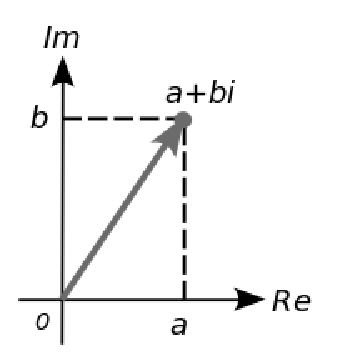
\includegraphics[width=0.45\textwidth,keepaspectratio]{img/ris_9_1}}\hspace*{0.05\textwidth}
%
\floatbox{figure}[.45\textwidth][\FBheight][b]
{\caption{Геометрическая интерпретация комплексно-сопряженного числа}
\label{ch09:refDrawing1}}
{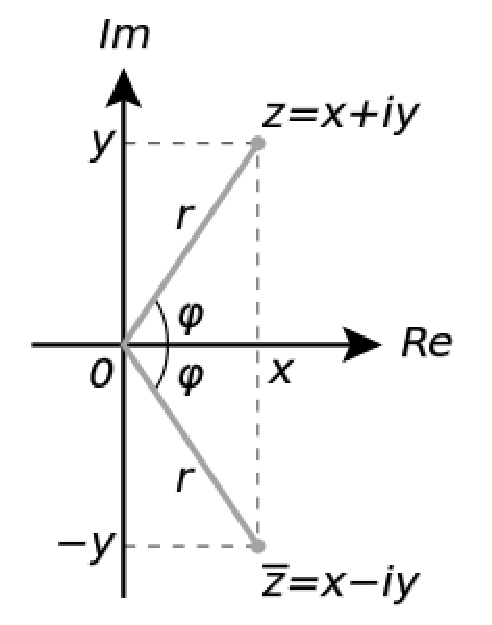
\includegraphics[width=0.45\textwidth,keepaspectratio]{img/ris_9_2}}
\end{floatrow}
\end{figure}


Следующая программа считывает информацию из файла \Sys{complex.dat} --- количество комплексных
чисел в переменную \Sys{n}, а сами комплексные числа в массив \Sys{p}.
 Затем происходит поиск комплексного числа с максимальным модулем в массиве \Sys{p}.

\begin{lstlisting}
#include <iostream>
#include <math.h>
using namespace std;
int main()
{
  struct complex
  {
    double Re;
    double Im;
  };
  complex *p;
  int i,n,nmax;
  double max;
  FILE *f;
  f=fopen("complex.dat","rb");
  fread(&n,sizeof(int),1,f);
  p=new complex[n];
  fread(p,sizeof(complex),n,f);
  //`Поиск комплексного числа с максимальным модулем`
  max=sqrt(p[0].Re*p[0].Re+p[0].Im*p[0].Im);
  for(i=1,nmax=0;i<n;i++)
    if (sqrt(p[i].Re*p[i].Re+p[i].Im*p[i].Im)>max)
    {
      max=sqrt(p[i].Re*p[i].Re+p[i].Im*p[i].Im);
      nmax=i;
    }
  cout<<"max="<<max<<"\t nmax="<<nmax<<endl;
  fclose(f);
  return 0;
}
\end{lstlisting}


\prg{Даны два комплексных числа  $z_1$  и  $z_2$. Выполнить
над ними \emph{основные операции}:}{ch09:prg1}
\begin{itemize}
\item сложение  $z_1+z_2$,
\item вычитание  $z_1-z_2$,
\item умножение  $z_1\cdot z_2$,
\item деление  $\frac{z_1}{z_2}$,
\item возведение в степень $n$  $z_1^n$,
\item извлечение корня $n$-й степени  $\sqrt[n]{z_1}$ 
\item вычисление комплексного сопряженного числа  $\bar{z}_1$.
\end{itemize}
\emph{Суммой двух комплексных чисел}  $z_1=a+i\cdot b$ и  $z_2=c+i\cdot d$ называется комплексное число $z=z_1+z_2=(a+c)+i\cdot (b+d)$.

\emph{Разностью двух комплексных чисел}  $z_1=a+i\cdot b$  и  $z_2=c+i\cdot d$ называется комплексное число  $z=z_1-z_2=(a-c)+i\cdot (b-d)$.

\emph{Произведением двух комплексных чисел}  $z_1=a+i\cdot b$  и  $z_2=c+i\cdot d$  называется
комплексное число
 $z=z_1\cdot {z_2}=(a\cdot c-b\cdot d)+i\cdot (b\cdot c+a\cdot d)$.

\emph{Частным двух комплексных чисел}  $z_1=a+i\cdot b$  и  $z_2=c+i\cdot d$ называется комплексное
число
\begin{equation*}
z=\frac{z_1}{z_2}=\frac{ac+bd}{c^2+d^2}+i\cdot {\frac{bc-ad}{c^2+d^2}}
\end{equation*}
Числом, \emph{сопряженным комплексному числу} 
$z=x+i\cdot y$,  называется число  $\bar{z}=x-i\cdot y$ (рис.~\ref{ch09:refDrawing1}).

Всякое комплексное число, записанное в \emph{алгебраической форме}  $z=x+i\cdot y$,
можно записать в \emph{тригонометрической}  $z=r(\cos \phi+i\cdot \sin \phi)$ или в
\emph{показательной форме}  $z=r\cdot e^{i\cdot \phi}$, где  $r=\sqrt{x^2+y^2}$ ---
\emph{модуль комплексного числа}  $z$,  $\phi=\arctan \frac{y}{x}$ --- его \emph{аргумент}
(рис.~\ref{ch09:refDrawing1}).

Для \emph{возведения в степень комплексного числа}, записанного в тригонометрической форме  $z=r(\cos
\phi+i\cdot \sin \phi)$, можно воспользоваться формулой Муавра

\begin{equation*}
z^n=r^n\cdot (\cos (n\cdot \phi)+i\cdot \sin (n\cdot \phi)).
\end{equation*}
Формула для \emph{извлечения корня} $n$-й \emph{степени} из комплексного
числа  $z=r\cdot (\cos \phi+i\cdot \sin \phi)$ имеет вид

 $\sqrt[n]z=\sqrt[n]z(\cos \frac{\phi+2\cdot \pi \cdot k}{n}+i\cdot \sin \frac{\phi+2\cdot \pi \cdot k}{n})$,

где  $n>1,k=0,1,\dots,n-1$.

Далее приведен текст программы реализующий алгоритм решения задачи~\ref{ch09:prg1}. В программе описаны две структуры для
работы с комплексными числами: структура \Sys{complex1} для представления комплексных чисел в
алгебраической форме (\Sys{Re} --- действительная часть комплексного числа, \Sys{Im} --- его
мнимая часть) и структура \Sys{complex2} для представления комплексных чисел в показательной или
тригонометрической форме (\Sys{Modul} --- модуль комплексного числа, \Sys{Argum} --- его
аргумент). Кроме того в программе созданы функции, реализующие основные действия над комплексными числами, переход
между различными формами представления комплексных чисел, а также ввод-вывод комплексных чисел. 
%Результат работы программы показан на рис.~\ref{ch09:refDrawing2}.

\begin{lstlisting}
#include <iostream>
#include <math.h>
using namespace std;
struct complex1
{
  float Re;
  float Im;
};
struct complex2
{
  float Modul;
  float Argum;
};
//`Ввод числа в алгебраической форме`
complex1 vvod1()
{
  complex1 temp;
  cout<<"`\Sys{Введите действительную часть числа}`\n";
  cin>>temp.Re;
  cout<<"`\Sys{Введите мнимую часть комплексного числа}`\n";
  cin>>temp.Im;
  return temp;
}
//`Ввод числа в тригонометрической или показательной форме`
complex2 vvod2()
{
  complex2 temp;
  cout<<"`\Sys{Введите модуль комплексного числа}`\n";
  cin>>temp.Modul;
  cout<<"`\Sys{Введите аргумент комплексного числа}`\n";
  cin>>temp.Argum;
  return temp;
}
//`Вывод числа в алгебраической форме`
void vivod(complex1 chislo)
{
  cout<<chislo.Re;
  if (chislo.Im>=0)
    cout<<" +"<<chislo.Im<<" i"<<endl;
  else 
    cout<<" "<<chislo.Im<<" i"<<endl;
}
//`Вывод  числа в тригонометрической форме`
void vivod(complex2 chislo)
{
  cout<<chislo.Modul<<" ( cos ("<<chislo.Argum<<") + i sin ("<<chislo.Argum<<"))"<<endl;
}
//`Перевод числа из тригонометрической формы в алгебраическую,`
//`pr определяет выводить или нет полученное число на экран.`
complex1 perevod(complex2 chislo, bool pr=false)
{
  complex1 temp;
  temp.Re=chislo.Modul*cos(chislo.Argum);
  temp.Im=chislo.Modul*sin(chislo.Argum);
  if (pr) vivod(temp);
  return temp;
}
//`Перевод числа из алгебраической формы в тригонометрическую,` 
//`pr определяет выводить или нет полученное число на экран.`
complex2 perevod(complex1 chislo, bool pr=false)
{
  complex2 temp;
  temp.Modul=sqrt(chislo.Re*chislo.Re+
  chislo.Im*chislo.Im);
  temp.Argum=atan(chislo.Im/chislo.Re);
  if (pr) vivod(temp);
  return temp;
}
//`Функция сложения двух чисел в алгебраической форме,`
//`pr определяет выводить или нет число на экран.`
complex1 plus1(complex1 chislo1,complex1 chislo2,bool pr=true)
{
  complex1 temp;
  temp.Re=chislo1.Re+chislo2.Re;
  temp.Im=chislo1.Im+chislo2.Im;
  if (pr) vivod(temp);
  return temp;
}
//`Функция вычитания двух чисел в алгебраической форме,`
//`pr определяет выводить или нет число на экран.`
complex1 minus1(complex1 chislo1,complex1 chislo2,bool pr=true)
{
  complex1 temp;
  temp.Re=chislo1.Re-chislo2.Re;
  temp.Im=chislo1.Im-chislo2.Im;
  if (pr) vivod(temp);
  return temp;
}
//`Функция умножения двух чисел в алгебраической форме,`
//`pr определяет выводить или нет число на экран.`
complex1 mult1(complex1 chislo1,complex1 chislo2,bool pr=true)
{
  complex1 temp;
  temp.Re=chislo1.Re*chislo2.Re-chislo1.Im*chislo2.Im;
  temp.Im=chislo1.Im*chislo2.Re+chislo1.Re*chislo2.Im;
  if (pr) vivod(temp);
  return temp;
}
//`Функция деления двух чисел в алгебраической форме,`
//`pr определяет выводить или нет число на экран.`
complex1 divide1(complex1 chislo1,complex1 chislo2,bool pr=true)
{
  complex1 temp;
  temp.Re=(chislo1.Re*chislo2.Re+chislo1.Im*chislo2.Im)/(chislo2.Re*chislo2.Re+chislo2.Im*chislo2.Im);
  temp.Im=(chislo1.Im*chislo2.Re-chislo1.Re*chislo2.Im)/(chislo2.Re*chislo2.Re+chislo2.Im*chislo2.Im);
  if (pr) vivod(temp);
  return temp;
}
//`Функция возведения комплексного числа в алгебраической форме` 
//`в целую степень n, pr определяет выводить или нет полученное число на экран.`
complex1 pow1(complex1 chislo1, int n, bool pr=true)
{
  complex1 temp;
  complex2 temp2;
  float p=1;
  int i=1;
  temp2=perevod(chislo1, true);//`Перевод числа в тригонометрическую форму.`
  for(;i<=n;p*=temp2.Modul,i++);
  temp.Re=p*cos(n*temp2.Argum);
  temp.Im=p*sin(n*temp2.Argum);
  if (pr) vivod(temp);
  return temp;
}
//`Функция извлечения корня степени n из комплексного числа`
//`в алгебраической форме, pr определяет выводить или нет`
//`полученные значения на экран. Функция возвращает ro и fi.`
void sqrtn1(complex1 chislo1, int n, float * ro, float * fi, bool pr=true)
{
  complex1 temp;
  complex2 temp2;
  int i=0;
  temp2=perevod(chislo1, true);//`Перевод числа в тригонометрическую форму.`
  *ro=pow(temp2.Modul, (float)1/n);
  *fi=temp2.Argum;
  if (pr)
  {
    for(i=0;i<n;i++)
    {
      cout<<i<<"`\Sys{-е значение корня}`\n";
      temp.Re=*ro*cos((*fi+2*M_PI*i)/n);
      temp.Im=*ro*sin((*fi+2*M_PI*i)/n);
      vivod(temp);
    }
  }
}
int main()
{
  complex1 chislo1, chislo2; //`Описание комплексных`
  complex1 chislo5; //`чисел в алгебраической форме.`
  complex2 chislo3, chislo4;//`Описание комплексных чисел в тригонометрической форме.`
  float ro1, fi1;
  chislo1=vvod1(); //`Ввод исходных данных`
  chislo2=vvod1();//`в алгебраической форме.`
  vivod(chislo1);//`Вывод исходных данных`
  vivod(chislo2);//`в алгебраической форме.`
  chislo3=perevod(chislo1,true); //`Перевод чисел`
  chislo4=perevod(chislo2,true);//`в тригонометрическую форму и вывод их на экран.`
  cout<<"`\Sys{Сумма чисел }`";
  chislo5=plus1(chislo1,chislo2,true);
  cout<<"`\Sys{Разность чисел }`";
  chislo5=minus1(chislo1,chislo2,true);
  cout<<"`\Sys{Произведение чисел }`";
  chislo5=mult1(chislo1,chislo2,true);
  cout<<"`\Sys{Частное чисел }`";
  chislo5=divide1(chislo1,chislo2,true);
  chislo5=pow1(chislo1,5,true); //`Возведение числа в пятую степень.`
  sqrtn1(chislo1, 5, &ro1, &fi1, true); //`Извлечение корня пятой степени.`
  return 0;
}
\end{lstlisting}

%\begin{figure}[ht]
%\begin{center}
%\caption{Результаты работы программы к задаче~\ref{ch09:prg1}}\label{ch09:refDrawing2}
Результаты работы программы к задаче~\ref{ch09:prg1}.
\begin{verbatim}
Введите действительную часть числа
5
Введите мнимую часть комплексного числа
-7
Введите действительную часть числа
11
Введите мнимую часть комплексного числа
1.85
5 -7 i
11 +1.85 i
8.60233 ( cos (-0.950547) + i sin (-0.950547))
11.1545 ( cos (0.166623) + i sin (0.166623))
Сумма чисел 16 -5.15 i
Разность чисел -6 -8.85 i
Произведение чисел 67.95 -67.75 i
Частное чисел 0.337961 -0.693203 i
8.60233 ( cos (-0.950547) + i sin (-0.950547))
1900 +47068 i
8.60233 ( cos (-0.950547) + i sin (-0.950547))
0-е значение корня
1.51018 -0.290608 i
1-е значение корня
0.743054 +1.34646 i
2-е значение корня
-1.05094 +1.12277 i
3-е значение корня
-1.39257 -0.652552 i
4-е значение корня
0.190285 -1.52606 i
\end{verbatim}
%\end{center}
%\end{figure}



\section[Библиотеки для работы с комплексными числами]{Библиотеки для работы с комплексными числами}
Работа с комплексными числами в \Sys{C++} реализована с помощью \index{Библиотека!комплексных чисел}\emph{библиотеки} 
\index{Библиотека!complex}\Sys{complex}. Подключение этой библиотеки дает
возможность применять операции $+$, $-$, \Sys{*}, $/$ для работы не только с вещественными, но и с комплексными числами.

Перед подключением библиотеки \Sys{complex} обязательно необходимо подключить библиотеку
\index{Библиотека!math.h}\Sys{math.h}.

Для \index{Библиотека!комплексных чисел!определение переменной}\emph{определения переменной 
типа комплексное число} используется оператор.

\Sys{complex <тип\_переменной> имя\_переменной;}

Здесь \Sys{тип\_переменной} --- это любой допустимый в \Sys{C++} числовой тип данных (\Sys{int},
\Sys{long int}, \Sys{double}, \Sys{float} и т.~д.), описывающий действительную и
мнимую части комплексного числа. Например,
\begin{lstlisting}
complex <float> x,y,z[5],*r;
complex <double> a;
complex <int> a,b,c;
\end{lstlisting}
Для \index{Библиотека!комплексных чисел!организация ввода-вывода}\emph{организации ввода-вывода
комплексных чисел} можно использовать библиотеку \index{Библиотека!iostream}\Sys{iostream} и стандартные
конструкции \Sys{cin}, \Sys{cout}. Например,
\begin{lstlisting}
#include <iostream>
#include <math.h>
#include <complex>
using namespace std;
int main(int argc, char **argv)
{
  complex <double> b, c;//`Описание комплексных чисел.`
  cout<<"b=";cin>>b;    //`Ввод комплексного числа b.`
  cout<<"c=";cin>>c;    //`Ввод комплексного числа c.`
  cout<<"b/c="<<b/c;    //`Вывод частного комплексных чисел`
  return 0;
}
\end{lstlisting}

В результате получим:
\begin{verbatim}
b=(1.24,-6.12)
c=(9.01,-11.22)
b/c=(0.385567,-0.199105)
\end{verbatim}
Обратите внимание, что при \emph{вводе комплексных чисел с клавиатуры} действительная и мнимая части
вводятся в скобках через запятую:

\Sys{(действительная\_часть, мнимая\_часть)}

Далее приведен пример \emph{присваивания комплексным переменным реальных значений} при их описании:
\begin{lstlisting}
complex <double> z (4.0, 1.0);
complex <int> r (4, -7);
\end{lstlisting}

Следующий пример демонстрирует как из двух числовых значений можно \emph{составить комплексное число}:
\begin{lstlisting}
#include <iostream>
#include <math.h>
#include <complex>
using namespace std;
int main(int argc, char **argv)
{
  double x1,y1;
  x1=-2.3;
  y1=8.1;
  complex <double> b (x1,y1); //`Формирование комплексного числа b` 
                              //`с действительной частью x1 и мнимой y1.`
  cout<<"b^2="<<b*b; //`Вывод квадрата комплексного числа.`
  return 0;
}
\end{lstlisting}

В табл. \ref{ch09:refTable0} представлены \index{Библиотека!комплексных чисел!основные
функции}\emph{основные математические функции} для работы с комплексными числами.
{\tabcolsep=0.3em\noindent\footnotesize
\begin{longtable}{|p{0.41\textwidth}|p{0.55\textwidth}|}
\caption{Основные функции комплексного аргумента}\label{ch09:refTable0}\\
\hline
\Emph{Прототип функции} &\Emph{Описание функции}\\
\hline \hline
\endfirsthead
\multicolumn{2}{c}%
{{\tablename\ \thetable{} --- продолжение}} \\
\hline
\Emph{Прототип функции} &\Emph{Описание функции}\\
\hline \hline
\endhead
\lstinline!double abs(complex z)! &Возвращает модуль комплексного числа~$z$.\\\hline
\lstinline!double arg(complex z)! &Возвращает значение аргумента комплексного числа~$z$.\\\hline
\lstinline!double asin(complex z)! &Возвращает арксинус комплексного числа~$z$\\\hline
\lstinline!double atan(complex z)! &Возвращает арктангенс комплексного числа~$z$ \\\hline
\lstinline!complex conj(complex z)! &Возвращает число комплексно сопряженное числу~$z$\\\hline
\lstinline!double cos(complex z)! &Возвращает косинус  комплексного числа~$z$.\\\hline
\lstinline!double cosh(complex z)! &Возвращает гиперболический косинус комплексного числа~$z$.\\\hline
\lstinline!double cosh(complex z)! &Возвращает экспоненту комплексного числа~$z$.\\\hline
\lstinline!double imag(complex z)! &Возвращает мнимую часть комплексного числа~$z$.\\\hline
\lstinline!double log(complex z)! &Возвращает натуральный логарифм комплексного числа~$z$.\\\hline
\lstinline!double log10(complex z)! &Возвращает десятичный логарифм комплексного числа~$z$.\\\hline
\lstinline!double norm(complex z)! &Возвращает квадрат модуля комплексного числа~$z$.\\\hline
\lstinline!complex pow(complex x, complex y)! &Возвращает степень комплексного числа~$z$.\\\hline
\lstinline!complex polar(double mag, double angle)! &Формирует комплексное число с модулем $mag$ и аргументом $angle$.\\\hline
\lstinline!double real(complex z)! &Возвращает действительную часть комплексного числа~$z$.\\\hline
\lstinline!complex sin(complex z)! &Возвращает синус комплексного числа~$z$.\\\hline
\lstinline!complex sinh(complex z)! &Возвращает гиперболический синус комплексного числа~$z$.\\\hline
\lstinline!complex sqrt(complex z)! &Возвращает квадратный корень комплексного числа~$z$.\\\hline
\lstinline!complex tan(complex z)! &Возвращает тангенс  комплексного числа~$z$.\\\hline
\lstinline!complex tan(complex z)! &Возвращает гиперболический тангенс комплексного числа~$z$.\\\hline
\end{longtable}
}

Далее приведен текст программы демонстрирующий работу с некоторыми функциями из табл.~\ref{ch09:refTable0}. 
%На рис.~\ref{ch09:prg3} 
После текста программы
показаны результаты ее работы.% программы.
\begin{lstlisting}
#include <iostream>
#include <math.h>
#include <complex>
using namespace std;
int main()
{
  complex <double> x (4, -6);
  complex <double> y (-7, 2);
  cout<<"x*y="<<x*y<<endl;
  cout<<"sin(x)*cos(y)="<<sin(x)*cos(y)<<endl;
  cout<<"conj(x)*ln(y)="<<conj(x)*log(y)<<endl;
  cout<<"sh(y)="<<sinh(y)<<endl;
  return 0;
}
\end{lstlisting}

%\begin{minipage}{12.965cm}
%{\centering\itshape
%Рис. {\refstepcounter{qwertya}\theqwertya\label{ch09:prg3}} Работа с математическими функциями комплексного аргумента
%\par}
% [Warning: Image ignored] % Unhandled or unsupported graphics:
%\includegraphics[scale=0.33]{glava9-img004}
%\end{minipage}
Результаты работы программы с некоторыми функциями комплексного аргумента
\begin{verbatim}
x*y=(-16,50)
sin(x)*cos(y)=(-747.159,10.2102)
conj(x)*ln(y)=(-9.23917,23.364)
sh(y)=(228.18,498.583)
\end{verbatim}

\prg{Вычислить  $y={(\sqrt{3}-i)}^{20}$, 
$z=\left(\frac{1+i\cdot \sqrt{3}}{1-i}\right)^{40}$.}{ch09:prg2}

Если провести аналитические преобразования, то получим следующее:

 $y=2^{19}\cdot (-1+i\cdot \sqrt{3})$,  $z=-2^{19}\cdot (1+i\cdot \sqrt{3})$.

Проверим эти вычисления с помощью программы на \Sys{C++}. 
%Как видно из рис. \ref{ch09:prg4} 
Результаты работы программы подтверждают аналитические вычисления.
%совпадают с аналитическими вычислениями.
\begin{lstlisting}
#include <iostream>
#include <math.h>
#include <complex>
using namespace std;
int main()
{
  complex <double> b(sqrt(3),-1),y;
  cout<<"b="<<b;
  y=pow(b,20);
  cout<<"y="<<y<<endl;
  cout<<real(y)/pow(2,19)<<"\t";
  cout<<imag(y)/pow(2,19)<<"\n";
  complex <double> a(1,sqrt(3)),c (1,-1),z;
  z=pow(a/c,40);
  cout<<"z="<<z<<endl;
  cout<<real(z)/pow(2,19)<<"\t";
  cout<<imag(z)/pow(2,19)<<"\n";
  return 0;
}
\end{lstlisting}
Результаты работы программы к задаче \ref{ch09:prg2}:
\begin{verbatim}
b=(1.73205,-1)y=(-524288,908093)
-1	1.73205
z=(-524288,-908093)
-1	-1.73205
\end{verbatim}


%\begin{minipage}{12.965cm}
%{\itshape
%Рис. {\refstepcounter{qwertya}\theqwertya\label{ch09:prg4}} Результаты работы программы к задаче \ref{ch09:prg2}}
% [Warning: Image ignored] % Unhandled or unsupported graphics:
%\includegraphics[scale=0.33]{glava9-img005}
%\end{minipage}

\index{Библиотека!комплексных чисел!операции с
массивами}\emph{Операции с массивами}, элементами которых являются комплексные числа, 
осуществляются также, как и с обычными
переменными. В качестве примера рассмотрим следующие задачи.

\prg{Написать программу умножения матриц комплексных чисел.
Матрицы $A$ и $B$ имеют вид:}{ch09:prg3}
{\noindent\scriptsize
$A=\left(\begin{array}{rrrr}1+2\cdot i&2+3\cdot i&3+1.54\cdot i&4-7.2\cdot i\\2+5\cdot i&3+7\cdot i&4+10\cdot i&5+14\cdot
i\\1.5+3.25\cdot i&1.7-3.94\cdot i&6.23+11.17\cdot i&-4.12+3.62\cdot i\end{array}\right)$,

\noindent $B=\left(\begin{array}{rrrrr}6.23-1.97\cdot i&0.19+0.22\cdot i&0.16+0.28\cdot i&3.4+1.95\cdot i&2.20-0.18\cdot
i\\0.22+0.29\cdot i&11+12\cdot i&6.72-1.13\cdot i&16+18\cdot i&34+66\cdot i\\5+1\cdot i&1.4-1.76\cdot i&4.5+2.3\cdot
i&296+700\cdot i&4.2+1.03\cdot i\\-3.4-2.61\cdot i&1+11\cdot i&2+23\cdot i&3-35\cdot i&4+47\cdot i\end{array}\right)$.
}

Пусть исходные данные хранятся в файле \Sys{abc.txt}. %(рис. \ref{ch09:prg5}).
Данные к задаче~\ref{ch09:prg3}\label{ch09:file0}, содержимое файла \Sys{abc.txt}:
\begin{verbatim}
3 4 5
(1,2) (2,3) (3,1.54) (4,-7.2)
(2,5) (3,7) (4,10) (5,14)
(1.5,3.25) (1.7,-3.94) (6.23,11.17) (-4.12,3.62)

(6.23,-1.97) (0.19,0.22) (0.16,0.28) (3.4,1.95) (2.20,-0.18)
(0.22,0.29) (11,12) (6.72,-1.13) (16,18) (34,66)
(5,1) (1.4,-1.76) (4.5,2.3) (296,700) (4.2,1.03)
(-3.14,-2.61) (1,11) (2,23) (3,-35) (4,47)
\end{verbatim}

%\begin{minipage}{13.414cm}
%{\itshape
%Рис. {\refstepcounter{qwertya}\theqwertya\label{ch09:prg5}} Данные к задаче \ref{ch09:refDrawing3}}
% [Warning: Image ignored] % Unhandled or unsupported graphics:
%\includegraphics[scale=0.33]{glava9-img006}
%\end{minipage}

Далее приведен текст программы реализующий алгоритм решения задачи~\ref{ch09:prg3}. 
%Результаты работы программы показаны на рис. \ref{ch09:prg6}.
\begin{lstlisting}
#include <iostream>
#include <fstream>
#include <math.h>
#include <complex>
using namespace std;
int main()
{
int i,j,p,N,M,K;
complex <float> **A,**B,**C;
ifstream f;
ofstream g;
f.open("abc.txt");
f>>N>>M>>K;
cout<<"N="<<N<<"\tM="<<M<<"\tK="<<K<<endl;
A=new complex <float> *[N];
for(i=0;i<N;A[i]=new complex <float> [M],i++);
B=new complex <float> *[M];
for(i=0;i<M;B[i]=new complex <float> [K],i++);
C=new complex <float> *[N];
for(i=0;i<N;C[i]=new complex <float> [K],i++);
for(i=0;i<N;i++)
  for(j=0;j<M;f>>A[i][j],j++);
cout<<"`\Sys{Матрица A}`\n";
for(i=0;i<N;cout<<endl,i++)
  for(j=0;j<M;cout<<A[i][j]<<"\t",j++);
for(i=0;i<M;i++)
  for(j=0;j<K;f>>B[i][j],j++);
cout<<"`\Sys{Матрица B}`\n";
for(i=0;i<M;cout<<endl,i++)
  for(j=0;j<K;cout<<B[i][j]<<"\t",j++);
for(i=0;i<N;i++)
  for(j=0;j<K;j++)
    for(C[i][j]=p=0;p<M;p++)
      C[i][j]+=A[i][p]*B[p][j];
f.close();
cout<<"`\Sys{Матрица C}`\n";
for(i=0;i<N;cout<<endl,i++)
  for(j=0;j<K;cout<<C[i][j]<<"\t",j++);
g.open("result.txt");
g<<"`\Sys{Матрица C=A*B}`\n";
for(i=0;i<N;g<<endl,i++)
  for(j=0;j<K;g<<C[i][j]<<"\t",j++);
g.close();
return 0;
}
\end{lstlisting}

%\begin{minipage}{15.956cm}
%{\itshape
%Рис. {\refstepcounter{qwertya}\theqwertya\label{ch09:prg6}} Результат умножения матриц из задачи \ref{ch09:refDrawing3}}
% [Warning: Image ignored] % Unhandled or unsupported graphics:
%\includegraphics[scale=0.33]{glava9-img007}
%\end{minipage}
Результат умножения матриц из задачи~\ref{ch09:prg3} (файл \Sys{result.txt}):

%{%\noindent\scriptsize
%\setverbatimfont{\normalfont\ttfamily\scriptsize}
\begin{verbatim}
Матрица C=A*B
(-8.152,34.598)   (75.8604,91.276)   (199.988,109.93)    (-452.5,2486.99)  (237.974,406.978)
(51.78,26.61)     (-177.52,190.35)   (-290.01,242.21)    (-5391.95,5813.9) (-986.2,783.76)
(59.6291,78.3851) (49.9912,-59.0193) (-82.8542,-50.3838) (-5763.7,7803.92) (149.766,-140.709)
\end{verbatim}
%}


\prg{Заданы матрицы $A$ и
$B$. Необходимо вычислить матрицу  $A^{-1}$  обратную к матрице  $A$, найти определитель
$|A|$  матрицы  $A$  и решить матричное уравнение  $A\cdot X=B$, где  $X=A^{-1}\cdot B$. Матрицы
$A$ и $B$ имеют вид:}{ch09:prg4}

 $A=\left(\begin{array}{rrr}1+2\cdot i&2+3\cdot i&3+1.54\cdot i\\2+5\cdot i&3+7\cdot i&4+10\cdot i\\1.5+3.25\cdot
i&1.7-3.94\cdot i&6.23+11.17\cdot i\end{array}\right)$,

 $B=\left(\begin{array}{rrr}1.5+3.25\cdot i&1.7-9.34\cdot i&6.23+11.17\cdot i\\0.11+8.22\cdot i&0.34-18.21\cdot i&1-7\cdot
i\\1+5\cdot i&7-13\cdot i&12+89\cdot i\end{array}\right)$.

Для хранения исходных данных создадим текстовый файл \Sys{abc2.txt} % (рис. \ref{ch09:prg7}).
следующего содержания:
\label{ch09:file1}\begin{verbatim}
3
(1,2) (2,3) (3,1.54)
(2,5) (3,7) (4,10)
(1.5,3.25) (1.7,-9.34) (6.23,11.17)

(1.5,3.25) (1.7,-9.34) (6.23,11.17)
(0.11,8.22) (0.34,-18.21) (1,-7)
(1,5) (7,-13) (12,89)
\end{verbatim}
%\begin{minipage}{13.758cm}
%{\itshape
%Рис. {\refstepcounter{qwertya}\theqwertya\label{ch09:prg7}} Исходные данные к задаче \ref{ch09:refDrawing4}}
% [Warning: Image ignored] % Unhandled or unsupported graphics:
%\includegraphics[scale=0.33]{glava9-img008}
%\end{minipage}

Текст программы, реализующий поставленную задачу представлен ниже. 
%Результаты работы программы показаны на рис.~\ref{ch09:prg8}.

\begin{lstlisting}
#include <iostream>
#include <fstream>
#include <math.h>
#include <complex>
using namespace std;
//`Решение СЛАУ с комплексными коэффициентами`
int SLAU(complex <float> **matrica_a,  int n, complex <float> *massiv_b, complex <float> *x)
{
int i,j,k,r;
complex <float> c,M,s;
float max;
complex <float> **a, *b;
a=new complex <float> *[n];
for(i=0;i<n;i++)
  a[i]=new complex <float>[n];
b=new complex <float> [n];
for(i=0;i<n;i++)
  for(j=0;j<n;j++)
    a[i][j]=matrica_a[i][j];
for(i=0;i<n;i++)
  b[i]=massiv_b[i];
for(k=0;k<n;k++)
{
  max= abs(a[k][k]);
  r=k;
  for(i=k+1;i<n;i++)
    if (abs(a[i][k])>max)
    {
      max=abs(a[i][k]);
      r=i;
    }
  for(j=0;j<n;j++)
  {
    c=a[k][j];
    a[k][j]=a[r][j];
    a[r][j]=c;
  }
  c=b[k];
  b[k]=b[r];
  b[r]=c;
  for(i=k+1;i<n;i++)
  {
    for(M=a[i][k]/a[k][k],j=k;j<n;j++)
      a[i][j]-=M*a[k][j];
    b[i]-=M*b[k];
  }
}
if (abs(a[n-1][n-1])==0)
  if(abs(b[n-1])==0)
    return -1;
  else return -2;
else
{
  for(i=n-1;i>=0;i--)
  {
    for(s=0,j=i+1;j<n;j++)
      s+=a[i][j]*x[j];
    x[i]=(b[i]-s)/a[i][i];
  }
return 0;
}
for(i=0;i<n;i++)
  delete [] a[i];
delete [] a;
delete [] b;
}
//`Вычисление обратной матрицы с комплексными коэффициентами`
int INVERSE(complex <float> **a, int n, complex <float> **y)
{
int i,j,res;
complex <float> *b, *x;
b=new complex <float> [n];
x=new complex <float> [n];
for(i=0;i<n;i++)
{
  for(j=0;j<n;j++)
    if (j==i)
      b[j]=1;
    else b[j]=0;
      res=SLAU(a,n,b,x);
  if (res!=0)
    break;
  else
    for(j=0;j<n;j++)
      y[j][i]=x[j];
}
delete [] x;
delete [] b;
if (res!=0)
  return -1;
else
  return 0;
}
//`Вычисление определителя матрицы с комплексными коэффициентами`
complex <float> determinant(complex <float> **matrica_a, int n)
{
int i,j,k,r;
complex <float> c,M,s,det=1;
complex <float> **a;
float max;
a=new complex <float> *[n];
for(i=0;i<n;i++)
  a[i]=new complex <float>[n];
for(i=0;i<n;i++)
  for(j=0;j<n;j++)
    a[i][j]=matrica_a[i][j];
for(k=0;k<n;k++)
{
  max=abs(a[k][k]);
  r=k;
  for(i=k+1;i<n;i++)
    if (abs(a[i][k])>max)
    {
      max=abs(a[i][k]);
      r=i;
    }
  if (r!=k) det=-det;
    for(j=0;j<n;j++)
    {
      c=a[k][j];
      a[k][j]=a[r][j];
      a[r][j]=c;
    }
  for(i=k+1;i<n;i++)
    for(M=a[i][k]/a[k][k],j=k;j<n;j++)
      a[i][j]-=M*a[k][j];
}
for(i=0;i<n;i++)
  det*=a[i][i];
return det;
for(i=0;i<n;i++)
  delete [] a[i];
delete [] a;
}
//`Умножение матриц с комплексными коэффициентами`
void umn (complex <float> **a, complex <float> **b, complex <float> **c, int n, int m, int k)
{
int i,j,p;
for(i=0;i<n;i++)
  for(j=0;j<k;j++)
    for(c[i][j]=p=0;p<m;p++)
      c[i][j]+=a[i][p]*b[p][j];
}
int main()
{
int i,j,N;
complex <float> **A,**B,**X, **Y;
ifstream f;
ofstream g;
f.open("abc2.txt");
f>>N;
cout<<"N="<<N<<endl;
A=new complex <float> *[N];
for(i=0;i<N;i++)
  A[i]=new complex <float> [N];
B=new complex <float> *[N];
for(i=0;i<N;i++)
  B[i]=new complex <float> [N];
X=new complex <float> *[N];
for(i=0;i<N;i++)
  X[i]=new complex <float> [N];
Y=new complex <float> *[N];
for(i=0;i<N;i++)
  Y[i]=new complex <float> [N];
for(i=0;i<N;i++)
  for(j=0;j<N;j++)
    f>>A[i][j];
cout<<"`\Sys{Матрица A}`\n";
for(i=0;i<N;cout<<endl,i++)
  for(j=0;j<N;j++)
    cout<<A[i][j]<<"\t";
for(i=0;i<N;i++)
  for(j=0;j<N;j++)
    f>>B[i][j];
cout<<"`\Sys{Матрица B}`\n";
for(i=0;i<N;cout<<endl,i++)
  for(j=0;j<N;j++)
    cout<<B[i][j]<<"\t";
if(!INVERSE(A, N, X))
{
  cout<<"`\Sys{Обратная матрица}`\n";
  for(i=0;i<N;cout<<endl,i++)
  for(j=0;j<N;j++)
    cout<<X[i][j]<<"\t";
}
else cout<<"`\Sys{Не существует обратной матрицы}`\n";
cout<<"`\Sys{Определитель}`="<<determinant(A,N);
umn(X,B,Y,N,N,N);
cout<<"\n `\Sys{Решение матричного уравнения}` \n";
for(i=0;i<N;cout<<endl,i++)
  for(j=0;j<N;j++)
    cout<<Y[i][j]<<"\t";
return 0;
}
\end{lstlisting}


%\begin{minipage}{12.965cm}
%{\itshape
%Рис. {\refstepcounter{qwertya}\theqwertya\label{ch09:prg8}} Результат работы программы к задаче \ref{ch09:refDrawing4}}
% [Warning: Image ignored] % Unhandled or unsupported graphics:
%\includegraphics[scale=0.33]{glava9-img009}
%\end{minipage}
Результат работы программы к задаче~\ref{ch09:prg4}:
\begin{verbatim}
N=3
Матрица A
(1,2)	(2,3)	(3,1.54)	
(2,5)	(3,7)	(4,10)	
(1.5,3.25)	(1.7,-9.34)	(6.23,11.17)	
Матрица B
(1.5,3.25)	(1.7,-9.34)	(6.23,11.17)	
(0.11,8.22)	(0.34,-18.21)	(1,-7)	
(1,5)	(7,-13)	(12,89)	
Обратная матрица
(-0.495047,-0.748993)	(0.325573,0.182901)	(-0.0340879,-0.0958618)	
(0.125154,0.0765918)	(-0.058179,-0.0728342)	(0.00208664,0.0685887)	
(0.157733,0.322512)	(-0.0859214,-0.127174)	(0.0143863,-0.000518244)	
Определитель=(7.50219,-208.261)
 Решение матричного уравнения 
(0.669246,-0.302366)	(-5.88068,-2.74393)	(15.0106,-16.4762)	
(0.190248,0.114415)	(0.488295,0.448942)	(-6.72319,3.21833)	
(0.241332,0.347549)	(1.02932,0.405788)	(-3.37716,5.51956)
\end{verbatim}

\section[Задачи для самостоятельного решения]{Задачи для самостоятельного решения}
\subsection[Структуры. Операции над комплексными числами]{Структуры. Операции над комплексными числами}
Разработать программу на языке \Sys{C++} для решения следующей задачи. Даны комплексные числа  $a=\alpha+\beta\cdot i$, 
$b=\gamma+\delta\cdot i$  и  $c=\lambda+\mu\cdot i$. Найти комплесное число  $d=\varphi+\psi\cdot i$  по формуле
представленной в табл. \ref{ch09:refTable1}.
\begin{longtable}{|r|p{0.5\textwidth}|}
\caption{Задания для решения задачи о комплексных числах} \label{ch09:refTable1}\\
\hline
\Emph{Вариант}&\Emph{Формула для вычислений}\\
\hline \hline
\endfirsthead
\multicolumn{2}{c}%
{{\tablename\ \thetable{} --- продолжение}} \\
\hline
\Emph{Вариант}&\Emph{Формула для вычислений}\\
\hline \hline
\endhead
1 &$d=a^2\cdot \frac{a+b}{a-b\cdot c}$\\\hline
2 &$d=a^2\cdot \frac{(a+b-c)}{b}$\\\hline
3 &$d=\frac{a^3\cdot b}{b+c}\cdot \left|a-b\right|$\\\hline
4 &$d=(a-c)^2\cdot \frac{(a+b)}{a}$\\\hline
5 &$d=\frac{a^2\cdot b}{a+c}\cdot (a-b)$\\\hline
6 &$d=(a+c)^2\cdot {\frac{(a-b)}{(a-c)}}$\\\hline
7 &$d=\frac{a\cdot b^2+c}{a-b}$\\\hline
8 &$d=(a+b-c)^2\cdot {\frac{b}{a}}$\\\hline
9 &$d=\frac{a\cdot b^3-c}{a+b}$\\\hline
10 &$d=(a+b-c)\cdot {\frac{b^2}{c}}$\\\hline
11 &$d=\frac{a^3\cdot b+c}{a-b}$\\\hline
12 &$d=\frac{(a^2+b-c^3)}{a}$\\\hline
13 &$d=\frac{a+b^2-c}{a+b+c}$\\\hline
14 &$d=\frac{(a+b^2-c)}{(a+b^2)}$\\\hline
15 &$d=\left(\frac{a+b+c}{a-b+c}\right)^2$\\\hline
16 &$d=(a-b-c)\cdot {\frac{(b+c)}{(b-c)}}$\\\hline
17 &$d=\left(\frac{a+b^3+c}{a-b^2-c}\right)$\\\hline
18 &$d=(a+b+c)\cdot {\frac{(b-a)}{(b-c)}}$\\\hline
19 &$d=\left(\frac{a-b-c}{a-b^2+c^3}\right)$\\\hline
20 &$d=\frac{(a^2-b+c)}{(b-c^3)}$\\\hline
21 &$d=\frac{(a+b+c)^2}{a-b-c}$\\\hline
22 &$d=(a+b+c)\cdot {\frac{(b+c)^2}{(b-c)^3}}$\\\hline
23 &$d=\frac{\left(a^2+b-c\right)\cdot a}{b}$\\\hline
24 &$d=\frac{(\frac{b}{c}+b\cdot c)}{(a-c)}$\\\hline
25 &$d=(a^2-\frac{b}{c})\cdot {\frac{(a+c)}{(a-c)}}$\\\hline
\end{longtable}

\subsection[Работа с библиотекой комплексных чисел]{Работа с библиотекой комплексных чисел}
Разработать программу на языке \Sys{C++} для решения следующей задачи:

\begin{enumerate}
\item Для заданной матрицы комплексных чисел $A(n\times n)$ найти  $B=3\cdot A^2+A^T$.
\item Для заданных матриц комплексных чисел $A(n\times n)$ и $B(n\times n)$ найти  $C=(2-3\cdot i)\cdot A\cdot B+B^T$.
\item Для заданных матриц комплексных чисел $A(n\times n)$ и $B(m\times m)$ найти  $C=\Delta\cdot A-A^2$, где  $\Delta=|B|$.
\item Для заданной матрицы комплексных чисел $A(n\times n)$ найти  $C=(3.2+1.8\cdot i)\cdot A^T-A^2$.
\item Для заданных матриц комплексных чисел $A(n \times n)$ и $B(n\times n)$ найти  $C=(3.5\cdot i)\cdot A\cdot B^T-B$.
\item Для заданных матриц комплексных чисел $A(n \times n)$ и $B(m \times m)$ найти  $C=\frac{\Delta}2\cdot A^T+A^2$, где  $\Delta=|B|$.
\item Для заданной матрицы комплексных чисел $D(k \times k)$ найти  $C=(3.2+1.8\cdot i)\cdot D^2-(5.2\cdot i)\cdot D^T$.
\item Для заданных матриц комплексных чисел $A(n \times n)$ и $B(n \times n)$ найти  $C=A\cdot B^T+A\cdot B$.
\item Для заданных матриц комплексных чисел $A(n \times n)$ и $B(m \times m)$ найти  $C=(\Delta\cdot A-A^T)\cdot A$, где  $\Delta=|B|$.
\item Для заданной матрицы комплексных чисел $F(m \times m)$ найти  $C=2.3\cdot (F^2+F)^T$.
\item Для заданных матриц комплексных чисел $A(n \times n)$ и $B(n \times n)$ найти  $C=(-2+3.5\cdot i)\cdot (A-B^T)^2$.
\item Для заданных матриц комплексных чисел $A(n \times n)$ и $B(m \times m)$ найти  $C=\Delta\cdot (A^2+A^T)$, где  $\Delta=|B|$.
\item Для заданной матрицы комплексных чисел $D(k \times k)$ найти  $C=(8.1\cdot i)\cdot (D^2-(1.2\cdot i)\cdot D^T)$.
\item Для заданных матриц комплексных чисел $A(n \times n)$ и $B(n \times n)$ найти  $C=(-1.5\cdot i)\cdot (A^T+B^T)^2$.
\item Для заданных матриц комплексных чисел $A(n \times n)$ и $B(m \times m)$ найти   $C=\Delta\cdot (A^T+A)^2$, где  $\Delta=|B|$.
\item Для заданной матрицы комплексных чисел $D(k \times k)$ найти $C=(D^T-(1.2\cdot i))\cdot D$.
\item Для заданных матриц комплексных чисел $A(n \times n)$ и $B(n \times n)$ найти  $C=(A^2+B^2)^T$.
\item Для заданных матриц комплексных чисел $A(n \times n)$ и $B(m \times m)$ найти  $C=\Delta\cdot (A^T+A)\cdot A$, где  $\Delta=|B|$.
\item Для заданной матрицы комплексных чисел $F(m \times m)$ найти  $C=-3.3\cdot (F^T-(2\cdot i)\cdot F)^2$. 
\item Для заданных матриц комплексных чисел $A(n \times n)$ и $B(n \times n)$ найти   $C=(A\cdot B+B\cdot A)^T$.
\item Для заданных матриц комплексных чисел $A(n \times n)$ и $B(m \times m)$ найти  $C=A-\Delta\cdot A\cdot A^T$, где  $\Delta=|B|$.
\item Для заданной матрицы комплексных чисел $F(m \times m)$ найти  $C=F^T+(3\cdot i)\cdot F^2$. 
\item Для заданных матриц комплексных чисел $A(n \times n)$ и $B(n \times n)$ найти   $C=((A+B)^2)^T$.
\item Для заданных матриц комплексных чисел $A(n \times n)$ и $B(m \times m)$ найти  $C=\Delta\cdot (A^2-A^T)$, где  $\Delta=|B|$.
\item Для заданной матрицы комплексных чисел $D(k \times k)$ найти $C=(D^T+(5-1.3\cdot i)\cdot D)^2$.
\end{enumerate}
